\begin{note}
	В теории функций одного переменного мы доказали замечательный результат, формулу Ньютона-Лейбница:
	\[
		\int_{[a; b]} F'(x)dx = F(b) - F(a)
	\]
	Неспроста подинтегральная функция написана в таком виде, ведь $dF(x) = F'(x)dx$, и это равенство можно интерпретировать как дифференциальную форму. Следующая часть текущего параграфа будет направлена на доказательство \textit{теоремы Стокса-Пуанкаре}, заявляющаяя в нашем случае такое равенство:
	\[
		\int_{[a; b]} dF = \int_{\vdelta([a; b])} F
	\]
\end{note}

\begin{definition}
	\textit{Цепью $k$-мерных кубов} называется формальная целочисленная комбинация $\sum_{i = 1}^N \alpha_i K_i$, где $\alpha_i \in \Z$, а $K_i$ --- соответствующий $k$-мерный куб в $\R^n$, $n \ge k$.
\end{definition}

\begin{anote}
	Формальность подразумевает, что это ни в коем случае не сумма множеств, а скорее просто кортеж.
\end{anote}

\begin{note}
	Грань $n$-мерного куба является просто $(n - 1)$-мерным кубом, живущим в гиперплоскости $\{x \in \R^n \colon x^j = \alpha\}$. Поэтому мы будем говорить, что каждой грани $K_\alpha^j$ соответствует свой экземпляр подпространства $E_j = \{x \in \R^n \colon x^j = 0\}$.
\end{note}

\begin{anote}
	Задать ориентацию для какой-то области $U \subset \R^n$ означает задать ориентацию на всём пространстве. Открытый куб --- тоже область.
\end{anote}

\begin{definition} (Правило ориентации)
	\begin{enumerate}
		\item Чтобы задать ориентацию для стандартного открытого куба $K$:
		\[
			K = \{x \in \R^n \colon \forall i \in \range{1}{n}\ 0 < x^i < 1\}
		\]
		будем считать $e_0$ положительным базисом (как это и было раньше).
		
		\item Рассматривая грань $K_\alpha^j$ со своим экземпляром $E_j$, зададим на этом подпространстве положительный ортонормированный базис. Выбор этого базиса произведём так, чтобы он был перестановкой векторов из $e_0 \bs \{e_j\}$ и если его кортеж дополнить слева выходящей из куба $K$ нормалью к $K_\alpha^j$, то получится положительно ориентированный базис в $\R^n$.
	\end{enumerate}
\end{definition}

\begin{anote}
	В случае произвольного куба нам нужен некоторый базис $e_0$, где каждый вектор является каким-то ориентированным ребром.
\end{anote}

\begin{anote}
	Если бы мы не обращали внимание на правило, а взяли для грани $K_\alpha^j$ базис $e_0$ без вектора $e_j^0$ (подразумевается не сама грань, естественно, а её экземпляр $E_j$), то в грани (в соответствующем $E_j$) была бы определена своя форма ориентированного объёма $V^j$:
	\[
		V^j = dx^1 \wedge \ldots \wedge dx^{j - 1} \wedge dx^{j + 1} \wedge \ldots \wedge dx^n
	\]
	Эту форму в такой записи можно понимать как форму в подпространстве, соответствующем грани $K_\alpha^j$, так и в $\R^n$.
\end{anote}

\textcolor{red}{Здесь надо картинку с кубом в трёхмерном пространстве}

\begin{proposition}
	Обозначим за $V_\alpha^j$ форму ориентированного объёма для грани $K_\alpha^j$. Тогда её можно записать следующим образом:
	\[
		V_\alpha^j = (-1)^{\alpha + j} dx^1 \wedge \ldots \wedge dx^{j - 1} \wedge dx^{j + 1} \wedge \ldots \wedge dx^n
	\]
\end{proposition}

\begin{proof}
	В силу того, как мы выбирали базис в грани $K_\alpha^j$, должно быть очевидным следующее равенство:
	\[
		V_\alpha^j = \eps_\alpha^j V^j,\ \eps_\alpha^j = \pm 1
	\]
	Заметим, что выходящей из куба нормалью к грани $K_\alpha^j$ можно всегда брать вектор $(-1)^{1 - \alpha}e_j^0$. Так как новый базис является просто перестановкой $e_0$ и мы знаем, что он положительно ориентирован, то должно быть справедливо равенство:
	\[
		(-1)^{1 - \alpha} dx^j \wedge \eps_\alpha^j V^j = V = dx^1 \wedge \ldots \wedge dx^n
	\]
	Остаётся расписать левую часть так, чтобы она отличалась от правой лишь видом коэффициента:
	\[
		(-1)^{1 - \alpha} \cdot \eps_\alpha^j \cdot (-1)^{j - 1} dx^1 \wedge \ldots \wedge dx^n = dx^1 \wedge \ldots dx^n \Lora (-1)^{-\alpha + j} \cdot \eps_\alpha^j;\ \eps_\alpha^j = (-1)^{-\alpha + j + 2\alpha} = (-1)^{\alpha + j}
	\]
\end{proof}

\begin{definition}
	\textit{Границей (краем) куба} $K$ назовём формальную сумму граней $K_\alpha^j$ с коэффициентами, соответствующими записи их форм ориентированного объёма:
	\[
		\vdelta K = \sum_{i \in \range{1}{n} \over {\alpha \in \{0, 1\}}} (-1)^{\alpha + i} K_\alpha^i
	\]
\end{definition}

\textcolor{red}{Тут нужно продемонстрировать границу $\vdelta([0; 1]) = \{1\} - \{0\}$ в одномерном случае}

\begin{theorem} (Стокса-Пуанкаре для стандартного куба)
	Если $\Omega$ --- гладкая $(n - 1)$-форма, заданная в окрестности стандартного куба $K$ $\textcolor{red}{^*}$, то имеет место формула:
	\[
		\int_K d\Omega = \int_{\vdelta K} \Omega
	\]
	где интеграл по границе куба нужно понимать следующим образом (интеграл по $K_\alpha^i$ нужно понимать как интеграл по $K \cap E_j$ --- некоторое множество в $(n - 1)$-мерном пространстве $E_j$, сопоставленное этой грани):
	\[
		\int_{\vdelta K} \Omega := \sum_{i \in \range{1}{n} \atop {\alpha \in \{0, 1\}}} (-1)^{\alpha + i} \int_{K_\alpha^i} \Omega
	\]
\end{theorem}

$\textcolor{red}{^*}$ Но есть нюанс, см. пункт 2 замечания в самом конце конспекта

\begin{proof}
	Поскольку обе части равенства зависят от $(n - 1)$-формы линейно, то достаточно проверить его для базисных форм с коэффициентами следующего вида:
	\[
		\Omega(x) = f_j(x) dx^1 \wedge \ldots \wedge dx^{j - 1} \wedge dx^{j + 1} \wedge \ldots \wedge dx^n
	\]
	Тогда запишем дифференциал формы:
	\[
		d\Omega(x) = df_j(x)dx^1 \wedge \ldots \wedge dx^{j - 1} \wedge dx^{j + 1} \wedge \ldots \wedge dx^n = (-1)^{j - 1}\pd{f_j}{x_j}(x) \underbrace{dx^1 \wedge \ldots \wedge dx^n}_{V(x)}
	\]
	По определению интеграла от дифференциальной формы мы имеем право записать следующее:
	\[
		\int_K d\Omega = (-1)^{j - 1}\int_K \pd{f_j}{x_j}(x)d\mu(x)
	\]
	По теореме Фубини этот интеграл можно свести к повторному. Тогда:
	\begin{multline*}
		\int_K \pd{f_j}{x_j}(x)d\mu(x) = \int_{E_j \cap K} d\mu(y) \int_{[0; 1]} \pd{f_j}{x_j} (y, x_j) d\mu(x_j) = \int_{E_j \cap K} (f_j(y, 1) - f_j(y, 0))d\mu(y) =
		\\
		\int_{K_1^j} f_j(y, 1)d\mu(y) - \int_{K_0^j} f_j(y, 0)d\mu(y)
	\end{multline*}
	где запись аргументов $(y, x_j)$ неформально, то есть по-хорошему $x_j$ должен быть на $j$-й позиции среди координат $y$. По итогу получили такое равенство:
	\[
		\int_K d\Omega = (-1)^{j - 1}\int_{K_1^j} f_j(y, 1)d\mu(y) + (-1)^j \int_{K_0^j} f_j(y, 0)d\mu(y)
	\]
	А теперь посмотрим на то, что такое интеграл по границе:
	\[
		\int_{\vdelta K} \Omega := \sum_{i \in \range{1}{n} \over {\alpha \in \{0, 1\}}} (-1)^{\alpha + i} \int_{K_\alpha^j} \Omega = (-1)^{j + 1} \int_{K_1^j} f_j(y, 1)d\mu(y) + (-1)^j \int_{K_0^j} f_j(y, 0)d\mu(y) = \int_K d\Omega
	\]
\end{proof}

\subsection{Интегрирование дифференциальных форм на элементарных многообразиях}

\begin{note}
	Если не оговорено явно другого, то при разговоре о пространствах $\R^n$, $\R^m$ подразумевается, что $n \ge m$, а $U$ --- область в $\R^m$.
\end{note}

\begin{definition}
	\textit{Диффеоморфизмом класса $C^k$} называется отображение $\phi \colon U \to V$, $U \subset \R^m$, $V \subset \R^n$, такое, что оно обладает следующими свойствами:
	\begin{enumerate}
		\item $\phi$ является биекцией
		
		\item $\phi$ непрерывно дифференцируемо на $U$ как минимум $k$ раз
		
		\item Матрица Якоби, соответствующая оператору $\phi$, имеет максимальный ранг в любой точке $U$
	\end{enumerate}
\end{definition}

\begin{note}
	Из этих трёх свойств и теоремы об обратной функции следует, что в случае $m = n$ это определение эквивалетно стандартному определению диффеоморфизма. Но более интересен следующий факт.
\end{note}

\begin{lemma} \label{main_diffeomorphism_lemma}
	Пусть $U, V \subset \R^m$, $W \subset R^n$, $\phi \colon U \to W$ и $\hat\phi \colon V \to W$ --- диффеоморфизмы гладкости $C^k$. Тогда $\pi := \hat\phi^{-1}\circ\phi \colon U \to V$ --- тоже диффеоморфизм гладкости $C^k$.
\end{lemma}

\begin{proof}
	Биективность очевидна. Нужно понять, как обстоят дела с дифференцированием: это не совсем тривиально, поскольку область определения $\hat\phi^{-1}$ не является открытым подмножеством $\R^n$ при $n > m$, поэтому обратная функция не подлежит дифференцированию. Однако мы можем применить теорему о неявной функции. 
	
	Сначала мы проверим дифференцируемость $\pi$ на $U$. Возьмём любую точку $u_0 \in U$ и обозначим $v_0 = \pi(u_0)$. Поскольку матрица Якоби $\hat\phi'$ имеет полный ранг в каждой точке, то в точке $v_0$ в ней найдутся $m$ линейно независимых строк с номерами $i_1, \ldots, i_m$. Заведём функцию $F = (F_1, \ldots, F_m) \colon U \times V \to \R^m$ по следующему правилу:
	\[
		\forall j = 1, \ldots, m \quad F_j(u, v) = \hat\phi_{i_j}(v) - \phi_{i_j}(u)
	\]
	Заметим, что $F$ удовлетворяет всем условиям теоремы о неявной функции в точке $(u_0, v_0)$: $F(u_0, v_0) = 0$, гладкость $F$ равна гладкости $\phi$ и $\hat\phi$, а матрица из частных производных $F$ по последним $m$ координатам в точке $(u_0, v_0)$ состоит из $m$ линейно независимых строк матрицы Якоби $\hat\phi'(v_0)$, то есть невырождена. Таким образом, в некоторой окрестности точки $u_0$ имеется дифференцируемая функция, однозначно задаваемая равенством $F(u, \pi(u)) = 0$. Но этому соотношению удовлетворяет $\pi$. Значит, $\pi$ дифференцируемо в $u_0$. И поскольку это верно для любой точки $u_0 \in U$, $\pi$ дифференцируемо на $U$.
	
	Теперь заметим, что у отображения $\pi$ есть обратное: $\pi^{-1} = \phi^{-1}\circ\hat\phi$, к которому можно применить аналогичные рассуждения и получить, что $\pi^{-1}$ тоже дифференцируемо на $V$. В этом случае, когда и сама функция, и обратная к ней дифференцируемы, можно продифференцировать тождество $\pi^{-1}(\pi(u)) = u$ и получить, что матрицы $\pi'$ и $(\pi^{-1})'$ всюду невырождены, то есть выполнено третье свойство диффеоморфизма.
	
	Также есть тождество $F(u, \pi(u)) = 0$ --- с его помощью нетрудно проверить по индукции, что $\pi$ имеет ту же гладкость, что и $F$, и частные производные $\pi$ имеют вид
	\[
		\pd{\pi_j^k}{u_{i_1}, \ldots, \partial u_{i_k}}(u) = \frac{P_k}{\ps{\det \pd{F}{v}}^{2k-1}}(u, \pi(u)),
	\]
	где $P_k$ --- некоторый многочлен от всевозможных частных производных функции $F$ до порядка $k$ включительно. Эту проверку мы опускаем. Это равенство имеет место в некоторой окрестности любой точки из $U$, то есть проверено второе свойство диффеоморфизма. 
	
\end{proof}

\begin{definition}
	\textit{Элементарным многообразием (клеткой)} в $\R^n$ назовём образ стандартного открытого куба $K \subset \R^m$ при диффеоморфизме $\phi$ класса $C^k$, определённого на некотором объемлющем кубе $K_\eps \supsetneq K$.
	
	При этом $\phi$ называется \textit{параметризацией}, а обратное отображение $\psi := \phi^{-1}$ называется \textit{координатным отображением}.
\end{definition}

\begin{center}
	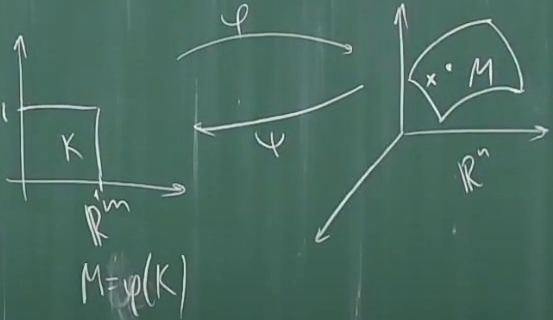
\includegraphics[width=0.4\textwidth]{images/cell.png}
\end{center}

\begin{note}
	Клетку, как и любое другое многообразие (они появятся позже), принято обозначать через $M$ (от английского слова manifold)
\end{note}

\begin{note}
	Чтобы включить класс диффеоморфизма в наименование клетки, её иногда называют \textit{клеткой класса $C^k$}. По умолчанию мы будем рассматривать класс $C^1$.
\end{note}

\begin{designation}
	Если не обговорено явно, считаем буквы $\phi$ и $\psi$ закреплёнными за соответствующими диффеоморфизмами, букву $M$ за клеткой, $K$ за параметризующим кубом, а $m$ и $n$ --- соответственно за размерностями куба и пространства, в которое вложена клетка. Кроме того, будет возникать много вопросов, связанных с независимостью от параметризацией. В связи с этим $\hat\phi$ будет обозначать другую параметризацию, $\hat\psi = \hat\phi^{-1}$ и $\pi = \hat\psi\circ\phi$ --- диффеоморфизм по лемме \ref{main_diffeomorphism_lemma}. Также положим $u = \psi(x)$ и $v = \hat\psi(x)$.
\end{designation}

\begin{definition}
	\textit{Касательным пространством} к клетке $M$ в точке $x$ называется линейное пространство $T(x)$, состоящее из всевозможных векторов вида $\phi'(u)\vv{H}$, $\vv H \in R^m$.
\end{definition}

\begin{center}
	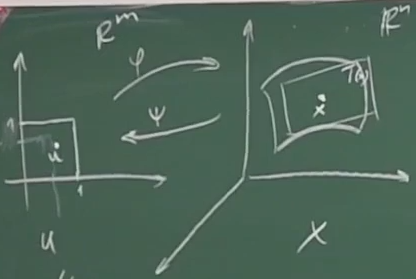
\includegraphics[width=0.4\textwidth]{images/cell_tangent.png}
\end{center}

\begin{lemma} \label{tangent_space_vs_param}
	Касательное пространство к клетке не зависит от параметризации.
\end{lemma}

\begin{proof}
	По определению нужно доказать, что совпадают множества $\phi'(u)\R^m$ и $\hat\phi'(v)\R^m$. Попробуем привести оба выражения к похожему виду:
	\begin{align*}
		&{\phi'(u)\R^m = (\hat\phi \circ \pi)'(u)\R^m = \hat\phi'(\pi(u))\pi'(u)\R^m}
		\\
		&{\hat\phi'(v)\R^m = \hat\phi'(\pi(u))\R^m}
	\end{align*}
	Как видим, отличие только в том, что сверху векторы из $\R^m$ дополнительно проходят через линейное преобразование, определяемое $\pi'(u)$. Но $\pi$ диффеоморфизм, поэтому ранг $\pi'(u)$ максимален, что равносильно $\R^m = \phi'(u)\R^m$. Значит, $\phi'(u)\R^m = \hat\phi'(v)\R^m$.
\end{proof}

\begin{definition}
	\textit{Касательным расслоением клетки} $M$ называется множество всех пар $(x, T(x))$.
\end{definition}

\begin{definition}
	Говорят, что \textit{дифференциальная форма задана на клетке $M$}, если она определена в каждой точке $x \in M$ и является в них кососимметричной линейной формой на $T(x)$.
\end{definition}

\begin{note}
	Тривиальный способ задать дифференциальную форму на клетке --- сужение: если $p$-форма $\Omega$ задана в окрестности $M$, то
	\[
		\Omega|_M(x)(\vv{G}_1, \ldots, \vv{G}_p) = \Omega(x)(\vv{G}_1, \ldots, \vv{G}_p),\ \ x \in M, \vv{G}_i \in T(x)
	\]
	Но даже если про объемлющее пространство мы ничего не знаем, можно перенести форму с параметризующего куба: 
\end{note}

\begin{definition} (от автора)
		Если $p$-форма $\Omega$ определена на открытом кубе $K$, то \textit{переносом формы $\Omega$ на клетку $M$ с помощью параметризации $\phi$} называется дифференциальная форма, заданная в каждой точке $x \in M$ на касательном пространстве $T(x)$ следующим образом:
		\[
			\psi^*\Omega(x)(\vv{G}_1, \ldots, \vv{G}_p) = \psi^*\Omega(x)(\phi'(u)\vv{H}_1, \ldots, \phi'(u)\vv{H}_p) := \Omega(u)(\vv{H}_1, \ldots, \vv{H}_p),\ \vv{G}_i \in T(x)
		\]
\end{definition}

\begin{note}
	Нетрудно видеть, что в случае $n = m$ это определение согласуется с переносом формы, введённым ранее, так как $\psi'(x)\phi'(u)\vv{H} = (\psi\circ\phi)'(u)\vv{H} = \vv{H}$.
\end{note}

\begin{note}
	Аналогичным образом мы можем перенести форму $\Pi$ из клетки $M$ на параметризующий куб $K$:
	\[
		\phi^*\Pi(u)(\vv{H}_1, \ldots, \vv{H}_p) = \Pi(\phi(u))(\phi'(u)\vv{H}_1, \ldots, \phi'(u)\vv{H}_p)
	\]
\end{note}

\begin{definition} (от автора)
	Дифференциальная форма $\Omega$, заданная на клетке $M$, называется \textit{гладкой}, если таковой является форма $\phi^* \Omega$.
\end{definition}

\begin{note}
	Параметризация не влияет на гладкость формы на клетке, поскольку $\phi^*\Omega(u) = \Omega(\phi(u)) = \hat\phi^*\Omega(\pi(u))$, где $\pi$ --- диффеоморфизм.
\end{note}

\begin{reminder}
	Мы опускаем первый аргумент $dx^i$ в силу его бессмысленности.
\end{reminder}

\begin{example}
	Покажем, что $dx^i|_M = \psi^*(d\phi^i)$, где $1 \le i \le n$. Возьмём любой вектор $\vv G = \phi'(u)\vv{H} \in T(x)$ и подставим его в левую часть:
	\[
		dx^i|_M(\vv{G}) = dx^i(\vv{G}) = dx^i(\phi'(u)\vv{H}) = \pd{\phi^i}{u_1}(u)H^1 + \ldots + \pd{\phi^i}{u_m}(u)H^m
	\]
	где $H^i$ --- соответствующая координата вектора $\vv{H}$. Если заменить $H^i$ на значение соответствующей 1-формы, то можно воспринимать $d\phi^i$ как $1$-форму и переписать это выражение так:
	\[
		\pd{\phi^i}{u_1}(u)du^1(\vv{H}) + \ldots + \pd{\phi^i}{u_m}(u)du^m(\vv{H}) = d\phi^i(u)(\vv{H}) = \psi^*(d\phi^i)(x)(\vv{G})
	\]
\end{example}

\begin{definition}
	Если $\Omega$ - гладкая $p$-форма на клетке $M = \phi(K)$, то \textit{дифференциалом формы на клетке} называется такая форма:
	\[
		d\Omega := \psi^*d(\phi^*\Omega)
	\]
	где $d(\phi^*\Omega)$ является внешним дифференциалом.
\end{definition}

\begin{lemma}
	Определенная операция дифференцирования форм не зависит от параметризации.
\end{lemma}

\begin{proof}
	Нам необходимо показать следующий факт:
	\[
		\psi^*d(\phi^*\Omega) = d\Omega = \hat{\psi}^*d(\hat{\phi}^*\Omega)
	\]
	С учётом формулы $\phi = \hat\phi\circ\pi$ выразим перенос $\phi^*\Omega$ через $\hat{\phi}^*$:
	\[
		\phi^*\Omega(u)(\vv{H}) = \Omega(\phi(u))(\phi'(u)\vv{H}) = \hat{\phi}^*\Omega(\pi(u))(\pi'(u)\vv{H}) = (\pi^* \circ \hat{\phi}^*)\Omega(u)(\vv{H}),
	\]
	где $\vv{H} = \vv{H}_1, \ldots, \vv{H}_p$, а $\hat\phi^*$ и $\pi^*$ понимаются как отображения между дифформами, определёнными на соответствующих областях.
	Аналогично получается равенство $\psi^*d(\phi^*\Omega) = (\hat{\psi}^* \circ (\pi^{-1})^*)d(\phi^*\Omega)$.
	Осталось расписать дифференциал и вспомнить про то, что при $n = m$ перенос формы коммутирует с дифференцированием:
	\[
		d\Omega = \psi^*d(\phi^*\Omega) = (\hat{\psi}^* \circ (\pi^{-1})^*)d((\pi^* \circ \hat{\phi}^*)\Omega) = (\hat{\psi}^* \circ (\pi^{-1})^* \circ \pi^*)d(\hat{\phi}^*\Omega) = \hat{\psi}^*d(\hat{\phi}^*\Omega)
	\]
\end{proof}

\begin{definition}
	\textit{Векторным полем на клетке} называется функция $A(x)$ такая, что $\forall x \in M\ A(x) \in T(x)$
\end{definition}

\begin{definition}
	Набор непрерывных векторных полей $\{e_i(x)\}_{i = 1}^m$ называется \textit{реп\'{е}ром для клетки} $M$, если в каждой точке многообразия этот набор образует базис пространства $T(x)$.
\end{definition}

\begin{example}
	Возьмём $\{h_i\}_{i=1}^m$ --- произвольный базис в пространстве $R^m$. Тогда репером может послужить $\{\phi'(u)h_i\}_{i=1}^m$. Это верно, поскольку $\phi'(u)h_i$ = $\phi'(\psi(x))h_i$ непрерывно зависит от $x$, а свойства базиса следуют уже из того, что ранг матрицы $\phi'(u)$ максимален.
\end{example}

\begin{definition}
	Пусть задана ориентация во всех касательных пространствах клетки $M$. Тогда, если $x, y \in M$ --- фиксированные произвольные точки, то касательные пространства $T(x)$ и $T(y)$ называются \textit{ориентированными согласованно}, если существует репер $\{e_i\}_{i = 1}^m$ такой, что базисы $\{e_i(x)\}_{i = 1}^m$ и $\{e_i(y)\}_{i = 1}^m$, являющиеся значениями этого репера в указанных точках, положительны в $T(x)$ и $T(y)$ соответственно.
\end{definition}

\begin{proposition}
	Все касательные пространства клетки могут быть ориентированы согласованно с помощью какого-либо репера.
\end{proposition}

\begin{proof}
	Возьмём любой репер $\{e_i\}_{i = 1}^m$ и зададим ориентацию на всех касательных пространствах $T(x)$, $x = \phi(u)$ таким образом, что базис $\{e_i(x)\}_{i = 1}^m$ является положительным.
\end{proof}

\begin{definition} (от автора)
	Клетка называется \textit{ориентированной}, если задана согласованная ориентация всех её касательных пространств.
\end{definition}

\begin{definition} (переформулировано автором)
	Параметризация $\phi$ ориентированной клетки $M$ называется \textit{положительной (отрицательной)}, если репер $\{\phi'(u)e_i\}_{i = 1}^m$ является положительным (отрицательным) для некоторого \underline{положительного} базиса $\{e_i\}_{i = 1}^m$, заданного на кубе $K$.
\end{definition}

\begin{definition}
	\textit{Интегралом от дифференциальной формы} $\Omega$, заданной на клетке $M = \phi(K)$, называется следующий интеграл:
	\[
		\int_M \Omega := \int_K \phi^*\Omega
	\]
\end{definition}

\begin{proposition}
	Модуль интеграла по клетке не зависит от параметризации.
\end{proposition}

\begin{proof}
	Снова вспомним формулу $\phi^* = \pi^* \circ \hat{\phi}^*$ и сошлёмся на то же утверждение для куба, доказанное в прошлом параграфе:
	\[
		\int_K \phi^*\Omega = \int_K (\pi^* \circ \hat{\phi}^*)\Omega = \pm \int_K \hat{\phi}^*\Omega
	\]
\end{proof}

\begin{anote}
	Доказывается, что модуль раскрывается с плюсом тогда и только тогда, когда "положительность" \ параметризации $\hat{\phi}$ та же, что и у $\phi$.
\end{anote}

\begin{definition}
	\textit{Границей (краем) клетки} $M$ называется формальная комбинация $\vdelta M := \sum_{i \in \range{1}{m} \atop {\alpha \in \{0, 1\}}} (-1)^{i + \alpha} M_\alpha^i$, где $M_\alpha^i = \phi(K_\alpha^i)$ для некоторой положительной параметризации $\phi$.
\end{definition}

\begin{note}
	Можно (но трудозатратно) доказать, что такое определение границы клетки не зависит от выбранной положительной параметризации. Мы же принимаем это утверждение без доказательства.
\end{note}

\begin{reminder}
	Напомню, что диффеоморфизм $\phi$ у нас определён на чуть большем кубе $K_\eps \supset K$. Ниже под окрестностью клетки $M$ можно подразумевать $\phi(K_\eps)$ --- на ней определены перенос формы и дифференцирование.
\end{reminder}

\begin{theorem} (Стокса-Пуанкаре для клетки)
	Пусть $\Omega$ --- гладкая $(m - 1)$-форма, заданная в окрестности клетки $M$. Тогда верно равенство:
	\[
		\int_M d\Omega = \int_{\vdelta M} \Omega,
	\]
	где
	\[
		\int_{\vdelta M} \Omega = \int_{\vdelta K} \phi^*\Omega
	\]
\end{theorem}

\begin{proof}
	\[
		\int_M d\Omega = \int_K \phi^* d\Omega = \int_K (\phi^* \circ \psi^*) d(\phi^* \Omega) = \int_K d(\phi^*\Omega) = \int_{\vdelta K} \phi^*\Omega = \int_{\vdelta M} \Omega
	\]
\end{proof}